Lo último sobre la experimentación es el análisis del modelado de un proceso de difusión.
Como se comentó en la Introducción (sección \ref{intro_difusion}), se construirá una matriz a partir de la fórmula allí dada.
La hipótesis es que, debido a la evolución de los $u_i$ en la fórmula $Au^{(k)} = u^{(k-1)}$ que es la que nos indica los valores, debería ocurrir que si partimos de un vector con valores mayores en el centro e inferiores a los lados, a medida que el proceso evoluciona los valores a los costados deberían comenzar a crecer ya que los valores centrales prestarían un porcentaje de sí mismos a sus vecinos.

Esta evolución se puede ver representada en el heatmap de la figura \ref{fig:heatmap_alpha_1}. Allí se observa cómo al principio hay una aglomeración de valores altos en el centro mientras que, a medida que avanza el proceso de difusión, los valores altos se van dispersando hasta llegar a un punto donde todos los valores son altamente similares.

\begin{figure}[H]   
      \centering
      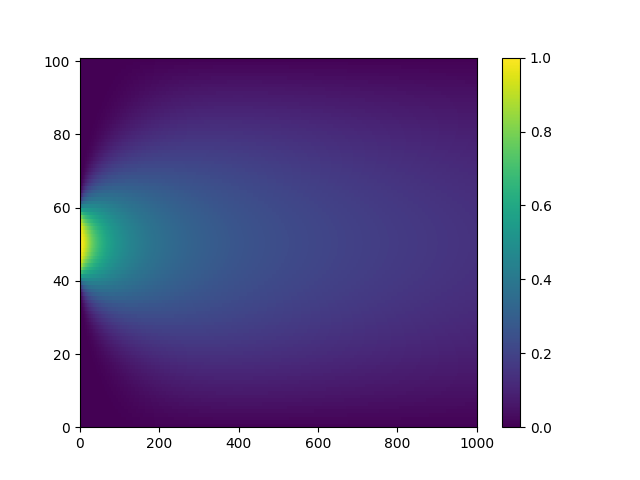
\includegraphics[scale=0.5]{graficos/difusion-alpha1.png}
      \caption{Heatmap para $\alpha = 1$}
      \label{fig:heatmap_alpha_1}
\end{figure}

Si variamos el $\alpha$ y se colocan otros valores como $\alpha = 0.1$ o $\alpha = 10$, se obtienen los resultados presentados en la figura \ref{fig:heatmap_diff_alpha}.

\begin{figure}[H]
      \centering
      \begin{subfigure}{.5\textwidth}
            \centering
            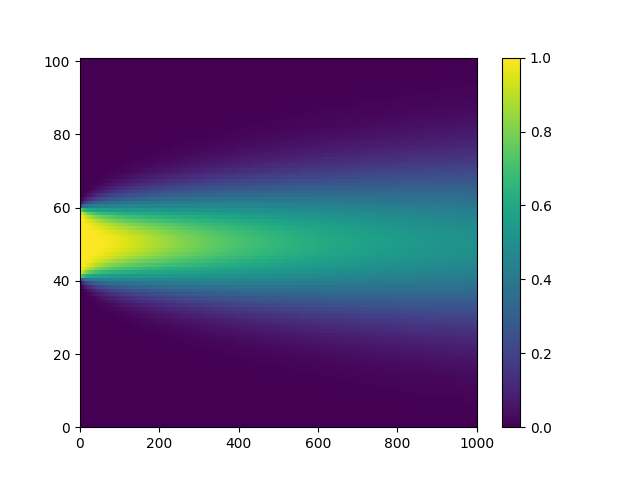
\includegraphics[width=\textwidth]{graficos/difusion-alpha01.png}
            \caption{Heatmap para $\alpha = 0.1$}
            \label{fig:heatmap_alpha_01}
      \end{subfigure}%
      \begin{subfigure}{.5\textwidth}
            \centering
            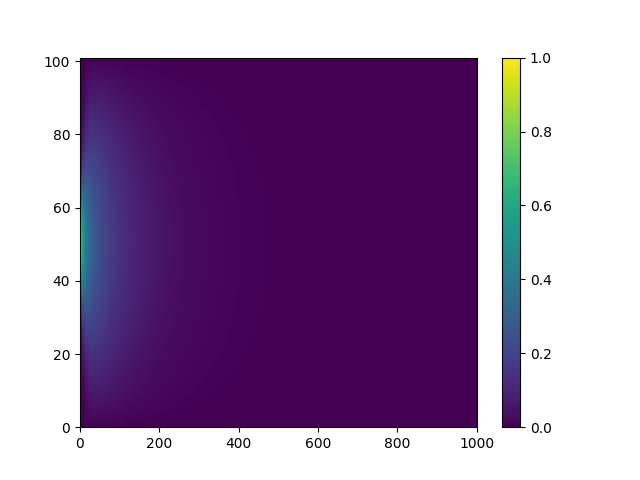
\includegraphics[width=\textwidth]{graficos/difusion-alpha10.png}
            \caption{Heatmap para $\alpha = 10$}
            \label{fig:heatmap_alpha_10}
      \end{subfigure}
      \caption{Heatmap con distintos valores de $\alpha$}
      \label{fig:heatmap_diff_alpha}
\end{figure}

Se puede observar que, mientras que para $\alpha=0.1$ la difusión del valor de los elementos centrales es menor y más lenta, por otro lado para $\alpha = 10$ los valores se dispersan mucho más rápido que en los casos anteriores.

Podemos concluir que $\alpha$ es muy importante al determinar el grado de difusión ya que su variación provoca resultados muy diferentes en la manera en la cual se dispersan los valores.
Para valores de $\alpha$ cercanos a $0$ obtenemos un foco centrado en los datos iniciales y una difusión mas lenta, pero para valores de $\alpha$ superiores a $1$ el foco se dispersa mucho más rápidamente.